\documentclass[10pt, oneside]{article}
\usepackage[a4paper, total={5.5in, 9in}]{geometry}
\usepackage[ngerman]{babel}

\usepackage{amsfonts}
\usepackage{dsfont}

\usepackage{blindtext}
\usepackage{titlesec}
\usepackage{amsmath}
\usepackage[hidelinks]{hyperref}
\usepackage{parskip}
\usepackage{graphicx}
\usepackage{longtable}
\usepackage[shortlabels]{enumitem}
\usepackage{multirow}
\usepackage{nccmath}
\usepackage{rotating}
\usepackage{makecell}
\usepackage{multicol}
\usepackage{capt-of}
\usepackage{csquotes}
\usepackage{amsfonts}
\usepackage{caption}

\captionsetup[table]{position=bottom}

\titleformat{\section}
    {\normalfont\Large\bfseries}{}{0pt}{}

\let\oldsection\section
\renewcommand{\section}{
  \renewcommand{\theequation}{\thesection.\arabic{equation}}
  \oldsection}
\let\oldsubsection\subsection
\renewcommand{\subsection}{
  \renewcommand{\theequation}{\thesubsection.\arabic{equation}}
  \oldsubsection}

\makeatletter
\renewcommand{\maketitle}{
    \bgroup
    \centering
    \par\LARGE\@title  \\[20pt]
    \par\large\@author \\[10pt]
    \par\large\@date
    \par
    \egroup
}
\makeatother


\title{Wahrscheinlichkeitstheorie und Statistik\\[5pt]\Large WiSe 2024/25\\[10pt]\Large L{\"o}sungen zu den Aufgaben 13, 16, 17, 18}
\author{Volodymyr But}
\date{Hochschule Trier}

% - - - - - - - - - - - - - - - - - - - - - - - - - - - - - - - - - - - - - - %

\begin{document}
\sloppy

\maketitle
\vspace{25px}

\section{Aufgabe 13}

\begin{enumerate}[1.]
    \item Wie viele M"oglichkeiten gibt es, 5 unterscheidbare Stifte auf 3 verschiedene
        Schubladen zu verteilen, wenn jede Schublade mehrere Stifte enthalten kann?

        \begin{equation*}
            \begin{aligned}
                |\text{Fa}^n_k(uD, mM)| &= |\text{Ur}^n_k(mR, mZ)| = \\[10pt]
                                        &= n^k = 3^5 = 243
            \end{aligned}
        \end{equation*}


    \item Wie viele M"oglichkeiten gibt es, 8 identische S"u{\ss}igkeiten auf 5
        verschiedene Teller zu verteilen, wobei ein Teller auch leer bleiben
        kann?

        \begin{equation*}
            \begin{aligned}
                |\text{Fa}^n_k(nuD, mM)| &= |\text{Ur}^n_k(oR, mZ)| = \\[10pt]
                                         &= \binom{n + k - 1}{k} = \binom{12}{8} = \\[5pt]
                                         &= \dfrac{12!}{8!(12 - 8)!} = \dfrac{12 \cdot 11 \cdot 10 \cdot 9}{4 \cdot 3 \cdot 2} = 495
            \end{aligned}
        \end{equation*}
\end{enumerate}

\section{Aufgabe 16}

In einer Lotterie werden 6 nummerierte Kugeln aus 49 Kugeln ungeordnet gezogen.
Wie viele Ziehung gibt es, welche die Zahlen 1, 2, 3 enthalten.

\textbf{L"osung.} Unter der Annahme, dass die Reihenfolge der Ziehungen unerheblich ist, lässt
sich feststellen, dass sich das Ergebnis, bei dem die ersten drei gezogenen
Kugeln die Zahlen 1, 2 und 3 enthalten, nicht von dem Ergebnis unterscheidet,
bei dem diese Kugeln in einer anderen Reihenfolge gezogen wurden. Es sollte
also gen"ugen, die Anzahl der Möglichkeiten zu berechnen, drei weitere
Kugeln zu ziehen, wenn man davon ausgeht, dass die drei Zielkugeln bereits
gezogen wurden.

\begin{equation*}
    \begin{aligned}
        |\text{Ur}^n_k(oR, oZ)| &= |\text{Fa}^n_k(nuD, oM)| = \\[5pt]
                                &= \binom{n}{k} = \binom{46}{3} = \\[5pt]
                                &= \dfrac{46!}{3!\cdot43!} = \dfrac{46 \cdot 45 \cdot 44}{3 \cdot 2} = 15180
    \end{aligned}
\end{equation*}

\pagebreak
\section{Aufgabe 18}

\begin{enumerate}[1.]
    \item Es seien $A := [0,1] \cup [2,3]$ und $B := [\dfrac{1}{2},
        \dfrac{3}{2}]$. 
        
        \begin{enumerate}[(a)]
            \item Skizzieren Sie den Graph von $f : [0,5] \longrightarrow
                \mathbb{R}$ mit $$f(x) := \mathds{1}_A(x) + \mathds{1}_B(x)$$

                \begin{figure}[h]
                    \centering
                    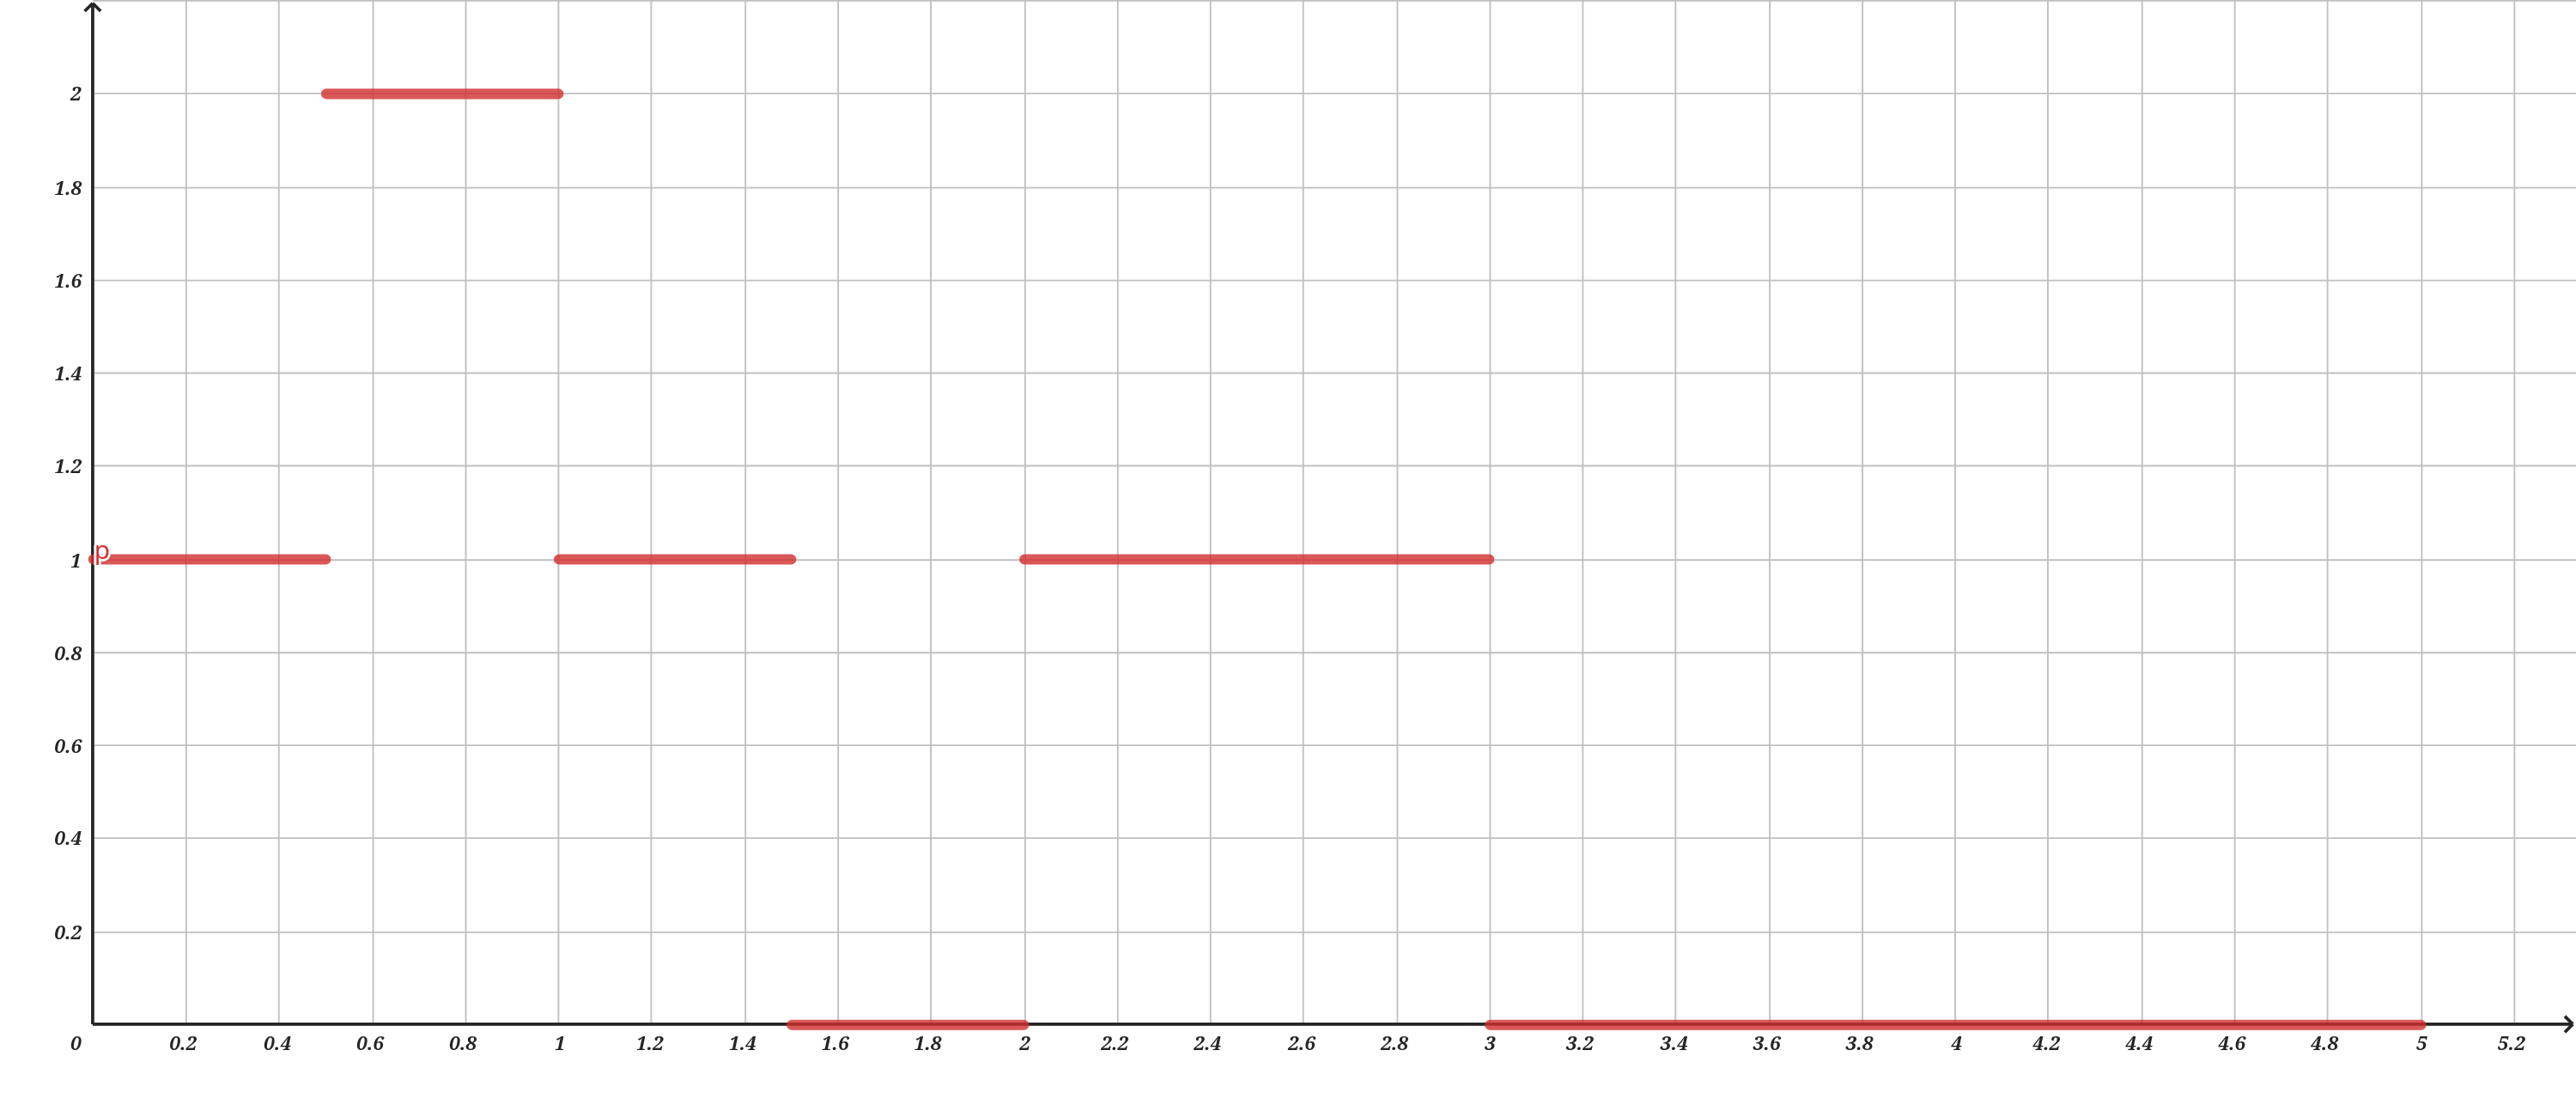
\includegraphics[width=0.9\textwidth]{./assets/18-01.png}
                    \caption{$f(x) := \mathds{1}_A(x) + \mathds{1}_B(x)$}
                \end{figure}

            \item Skizzieren Sie den Graph von $g: [0, 5] \longrightarrow
                \mathbb{R}$ mit $$g(x) := \mathds{1}_A(x) - \mathds{1}_B(x)$$

                \begin{figure}[h]
                    \centering
                    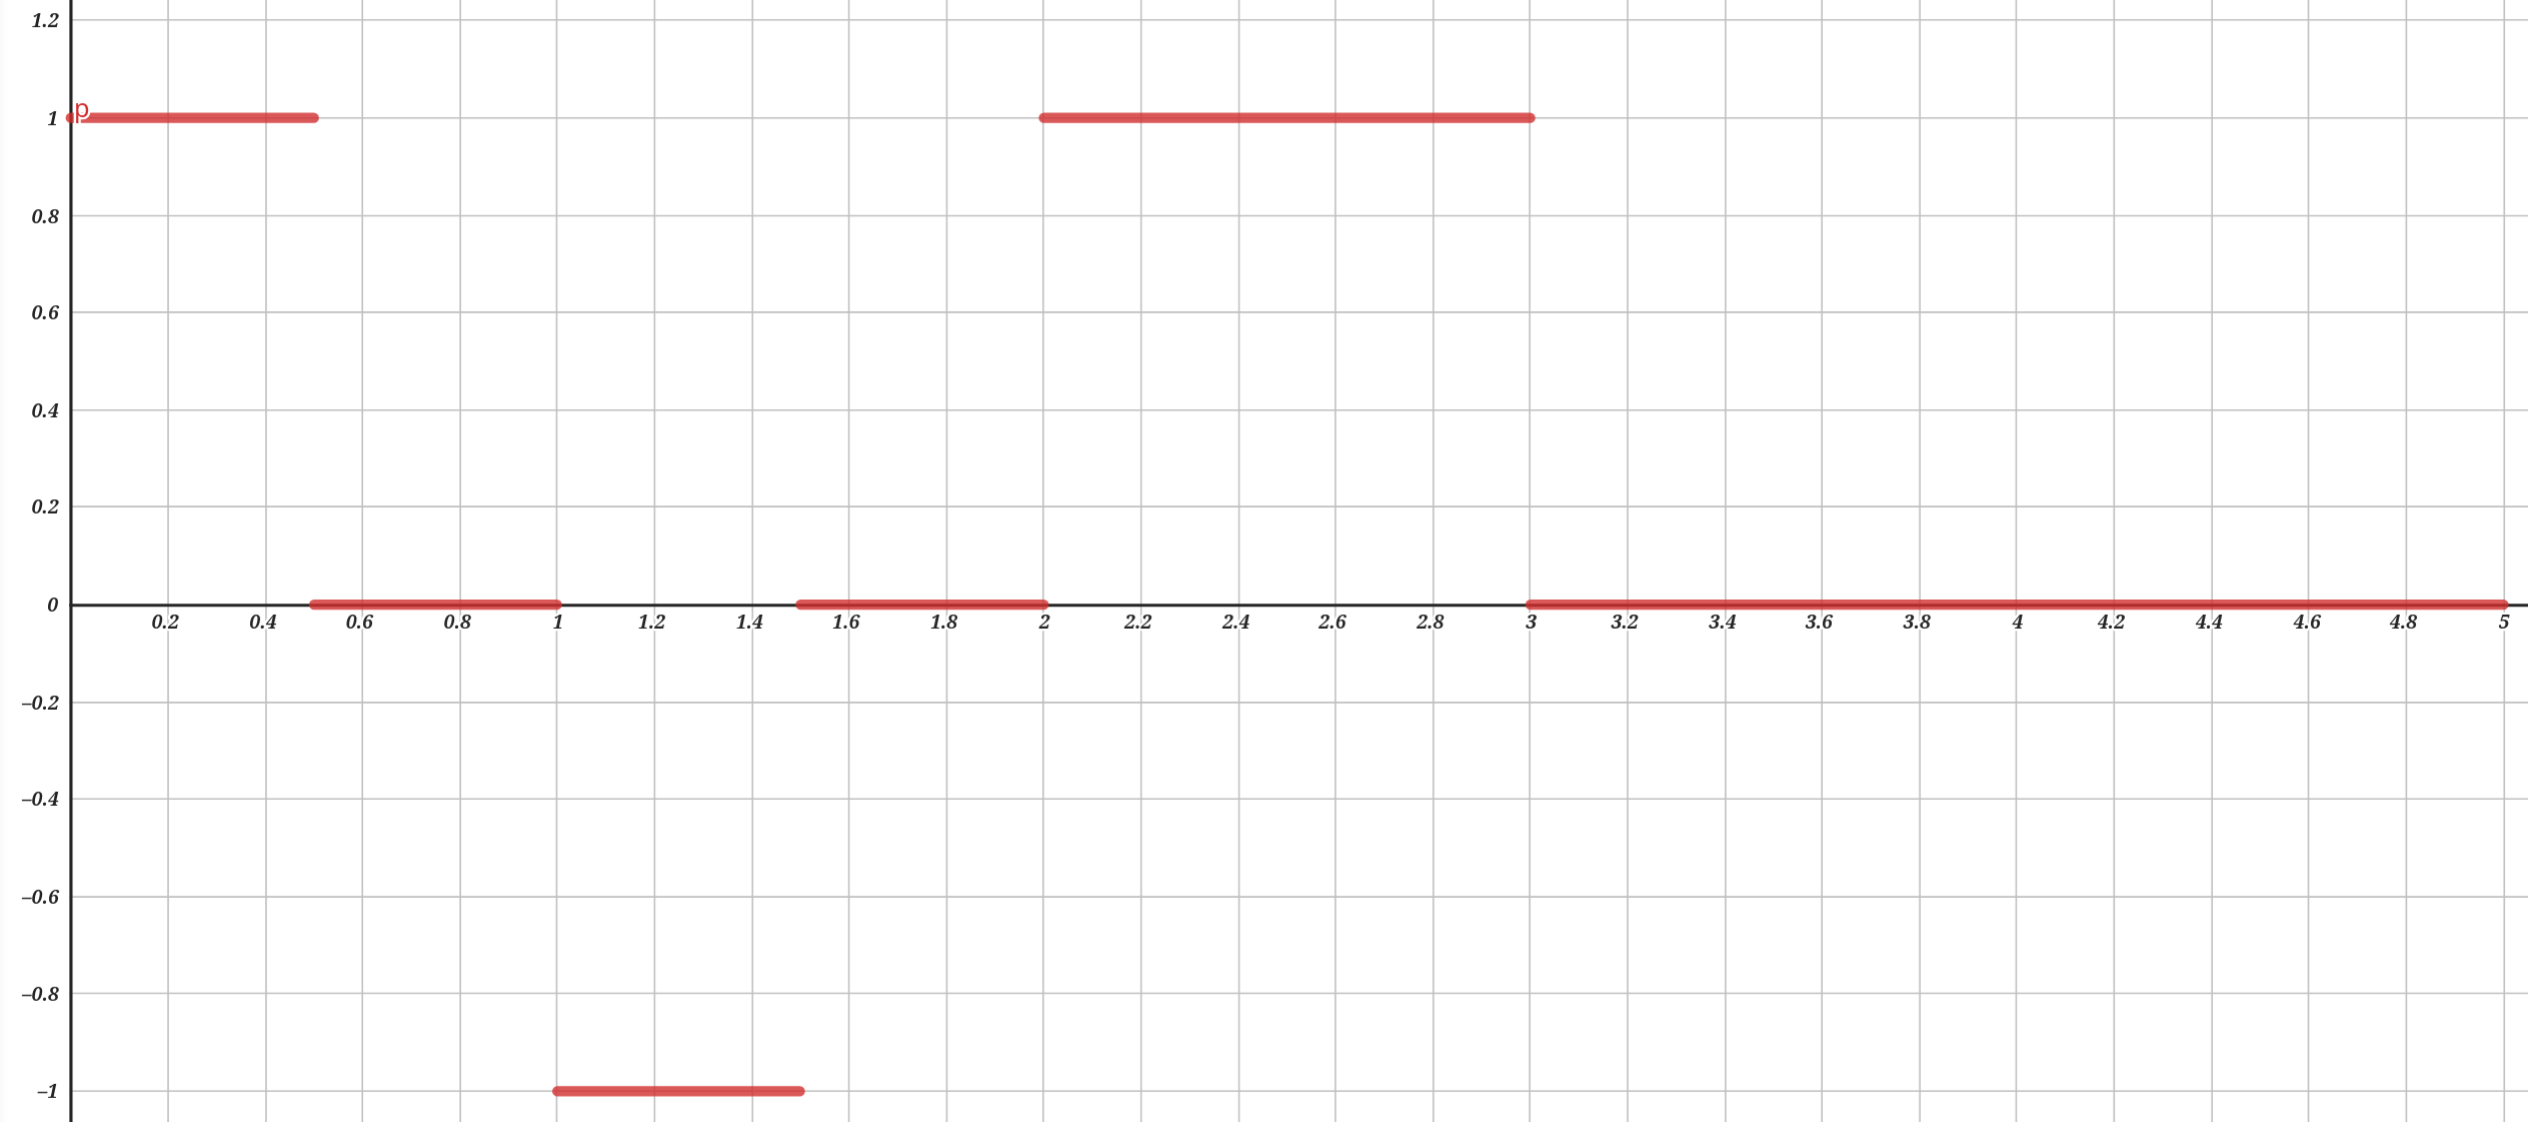
\includegraphics[width=0.9\textwidth]{./assets/18-02.png}
                    \caption{$f(x) := \mathds{1}_A(x) - \mathds{1}_B(x)$}
                \end{figure}
        \end{enumerate}
\end{enumerate}


\end{document}
